\documentclass[11pt, oneside]{article}
\usepackage[bottom=2.5cm,top=2.5cm]{geometry}
\geometry{a4paper}
\usepackage{graphicx}
\usepackage{amssymb}
\usepackage[utf8]{inputenc}
\usepackage[brazil]{babel}
\usepackage{color}
\usepackage{float}
\usepackage{hyperref}
\bibliographystyle{apalike}
\usepackage{indentfirst}

\title{Briefing Clima Espacial}
\date{2022/04/25}

\begin{document}
\maketitle 

 \section{Sol} 
 \subsection{Responsável: José Cecatto}

05/02 – Fast (=$<$ 500 km/s) wind stream; 4 CME c.h.c. toward the Earth; \\ 05/03 – 1 M1, 1 X1 and radio blackout ; Fast (=$<$ 450 km/s) wind stream; 8 CME c.h.c. toward the Earth; \\ 05/04 – 2 M5+ flares, 3 M1 and radio blackout; No fast wind stream; 8 CME c.h.c. toward the Earth; \\ 05/05 – 2 M1 flares; No fast wind stream; 5 CME c.h.c. toward the Earth; \\ 05/06 – No fast wind stream; 5 CME c.h.c. toward the Earth; \\ 05/07 – No fast wind stream; 2 CME c.h.c. toward the Earth; \\ 05/08 – No fast wind stream; 4 CME c.h.c. toward the Earth; \\ 05/09 – No fast wind stream; 1 CME c.h.c. toward the Earth; \\ Prev.: No fast wind up to May 12; for the next 2 days relatively low (30\% M, 5\% X) probability of M / X flares; also, \\ occasionally other CME can present component toward the Earth. \\ c.h.c. – can have a component\section{Cinturões de Radiação} 
 \subsection{Responsável: Ligia Alves da Silva} 
 
\begin{figure}[H]
    
                        \centering
   
                             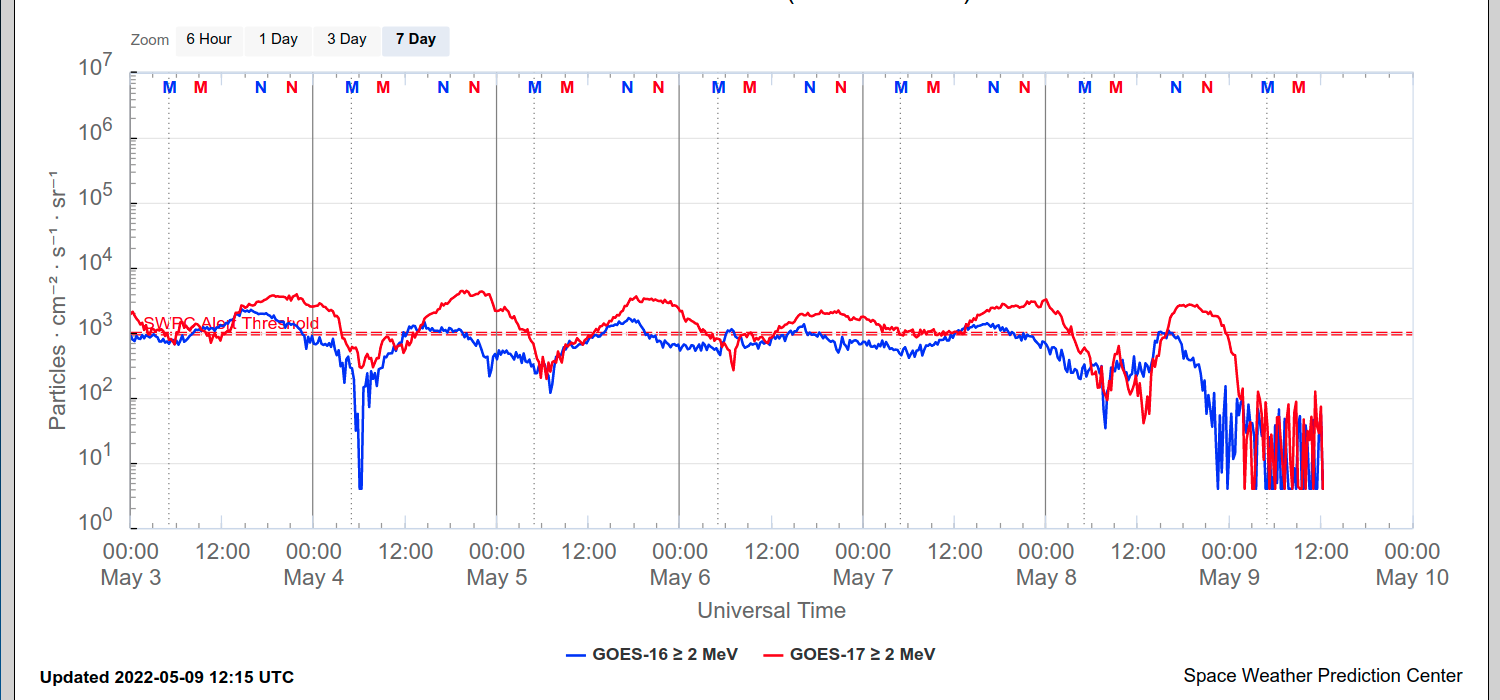
\includegraphics[width=14cm]{./figures//figureRadBelts_0.png}

                             \caption{ Fluxo de elétrons de alta energia (> 2MeV) obtido a partir dos satélites GOES-16 e GOES-17. Fonte}
                        \end{figure}

                     \begin{figure}[H]
    
                        \centering
   
                             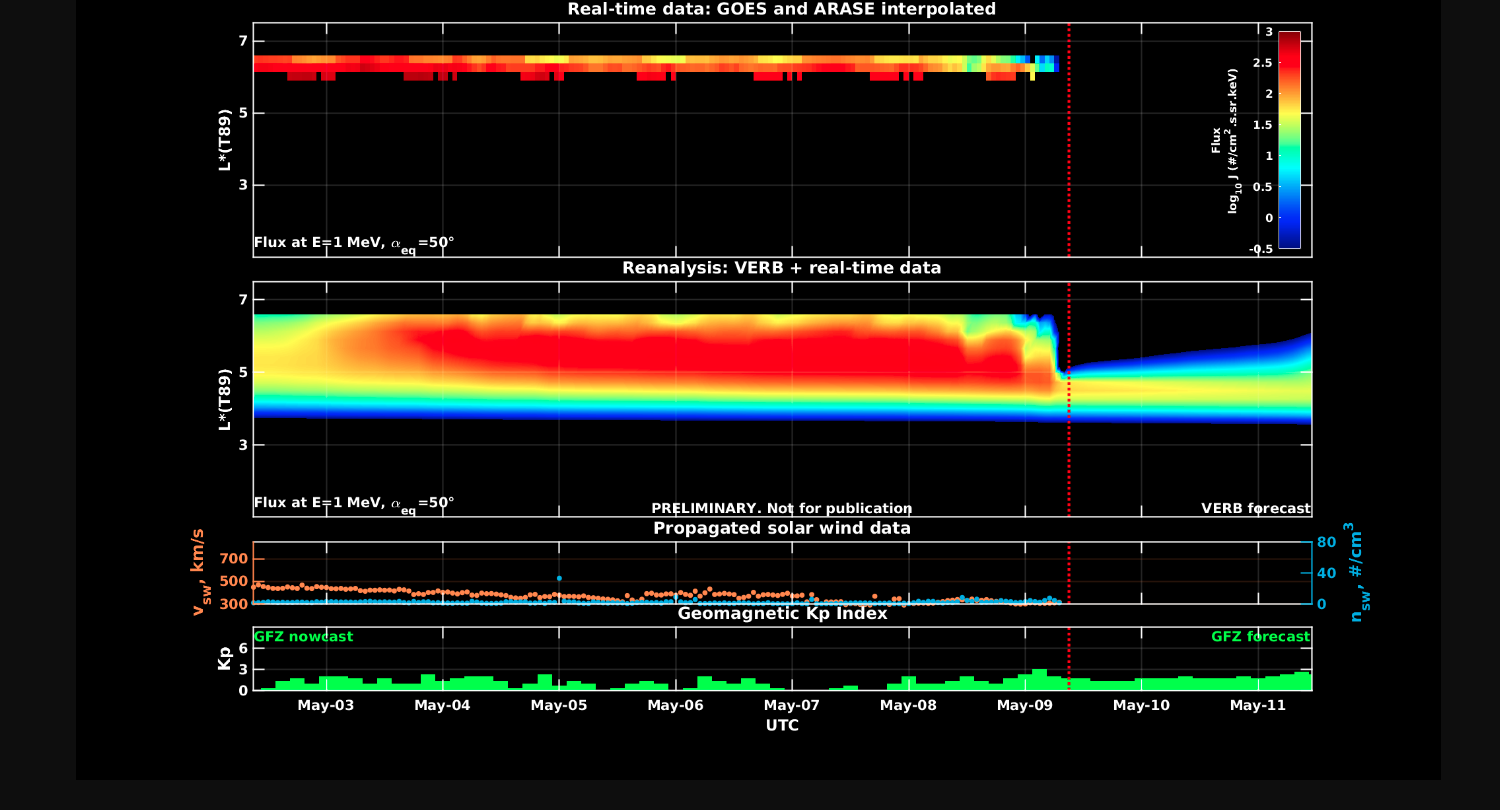
\includegraphics[width=14cm]{./figures//figureRadBelts_1.png}

                             \caption{ Dados de fluxo de elétrons de alta energia (reais e interpolados) obtidos a partir dos satélites ARASE, GOES-16, GOES-17. Dados reanalisados a partir do VERB code e do fluxo de elétrons interpolados. Dados da velocidade do vento solar e densidade de prótons obtidos a partir do satélite ACE. Fonte}
                        \end{figure}

                     O fluxo de Elétrons de alta energia (>2 MeV) na borda do cinturão de radiação externo obtidos a partir do satélite geoestacionário GOES-16 e GOES-17 (Figura 1) apresenta-se estável em torno do limiar de 103 partículas/(cm2 s sr) durante toda a semana de analise. Três diminuições de fluxo de elétrons são observadas nos dias 4, 8 e 9 de maio, respectivamente. A primeira diminuição é consideravelmente rápida, retornando ao limiar de 103 partículas/(cm2 s sr). A segunda diminuição atinge aproximadamente 1 ordem de grandeza e persiste por mais de 9 horas. A terceira diminuição de fluxo de elétrons atinge aproximadamente 2 ordens de grandeza e persiste até o último registro. 

Os dados dos satélites ARASE, GOES-16 e GOES-17 são analisados e interpolados para que a variabilidade do fluxo de elétrons de alta energia (1 MeV) seja observada em todo o cinturão externo de radiação (Figura 2). Adicionalmente o VERB code reconstrói este fluxo considerando a difusão radial por ondas Ultra Low Frequency (ULF). A simulação (VERB code) mostra que a primeira diminuição de fluxo de elétrons ocorre apenas na borda do cinturão, a segunda atinge L-shell = 6.0, e a terceira atinge L-shell = 5.0. Estas variabilidades no fluxo de elétrons ocorreram concomitantes a chegada de estruturas do vento solar e atividades de ondas ULF. Contudo, é importante salientar que os dados do satélite ARASE não estão disponíveis para a semana em análise, para confirmação do nível de L-shell destas variabilidades no fluxo de elétrons.



\section{Ondas ULF} 
 \subsection{Responsável: José Paulo Marchezi} 
 
\begin{figure}[H]
    
                        \centering
   
                             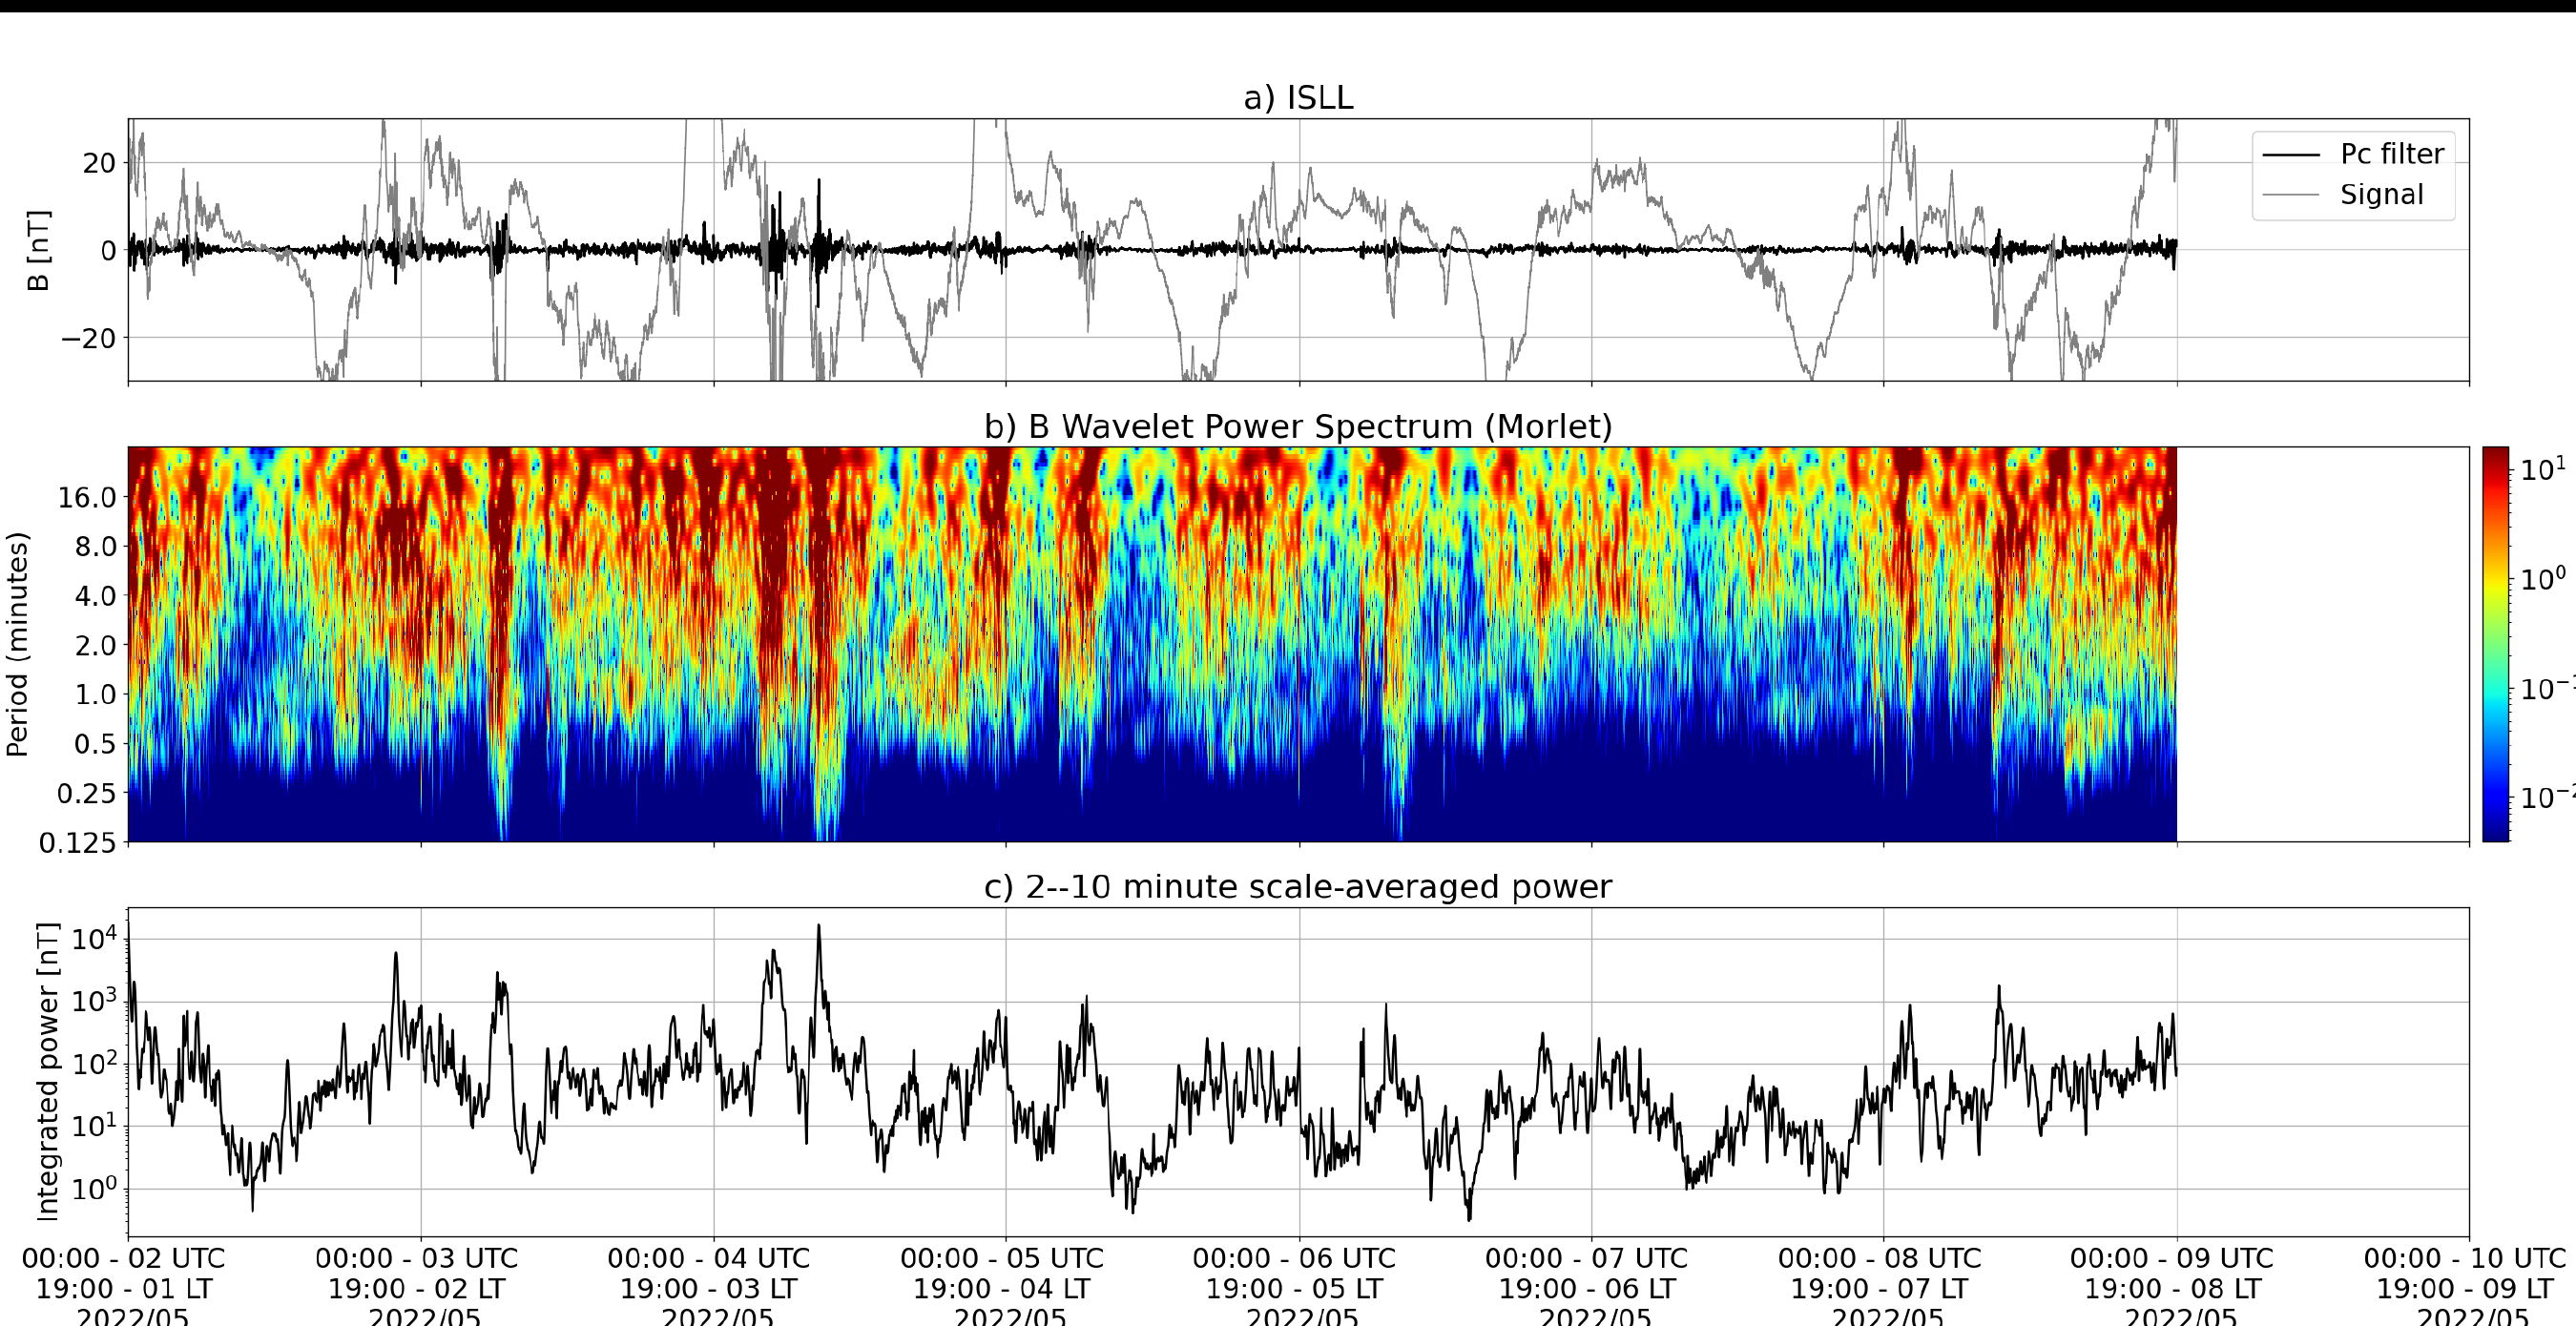
\includegraphics[width=14cm]{./figures//figureULF_0.png}

                             \caption{a) sinal do campo magnético total 
                              medido na Estação ISLL da rede CARISMA em cinza, 
                              junto com a flutuação na faixa de Pc5 em preto. b) 
                              Espectro de potência wavelet do sinal filtrado. c) 
                              Média da potência espectral nas faixas de 2 a 10 minutos 
                              (ondas ULF).}
                        \end{figure}

                     \begin{figure}[H]
    
                        \centering
   
                             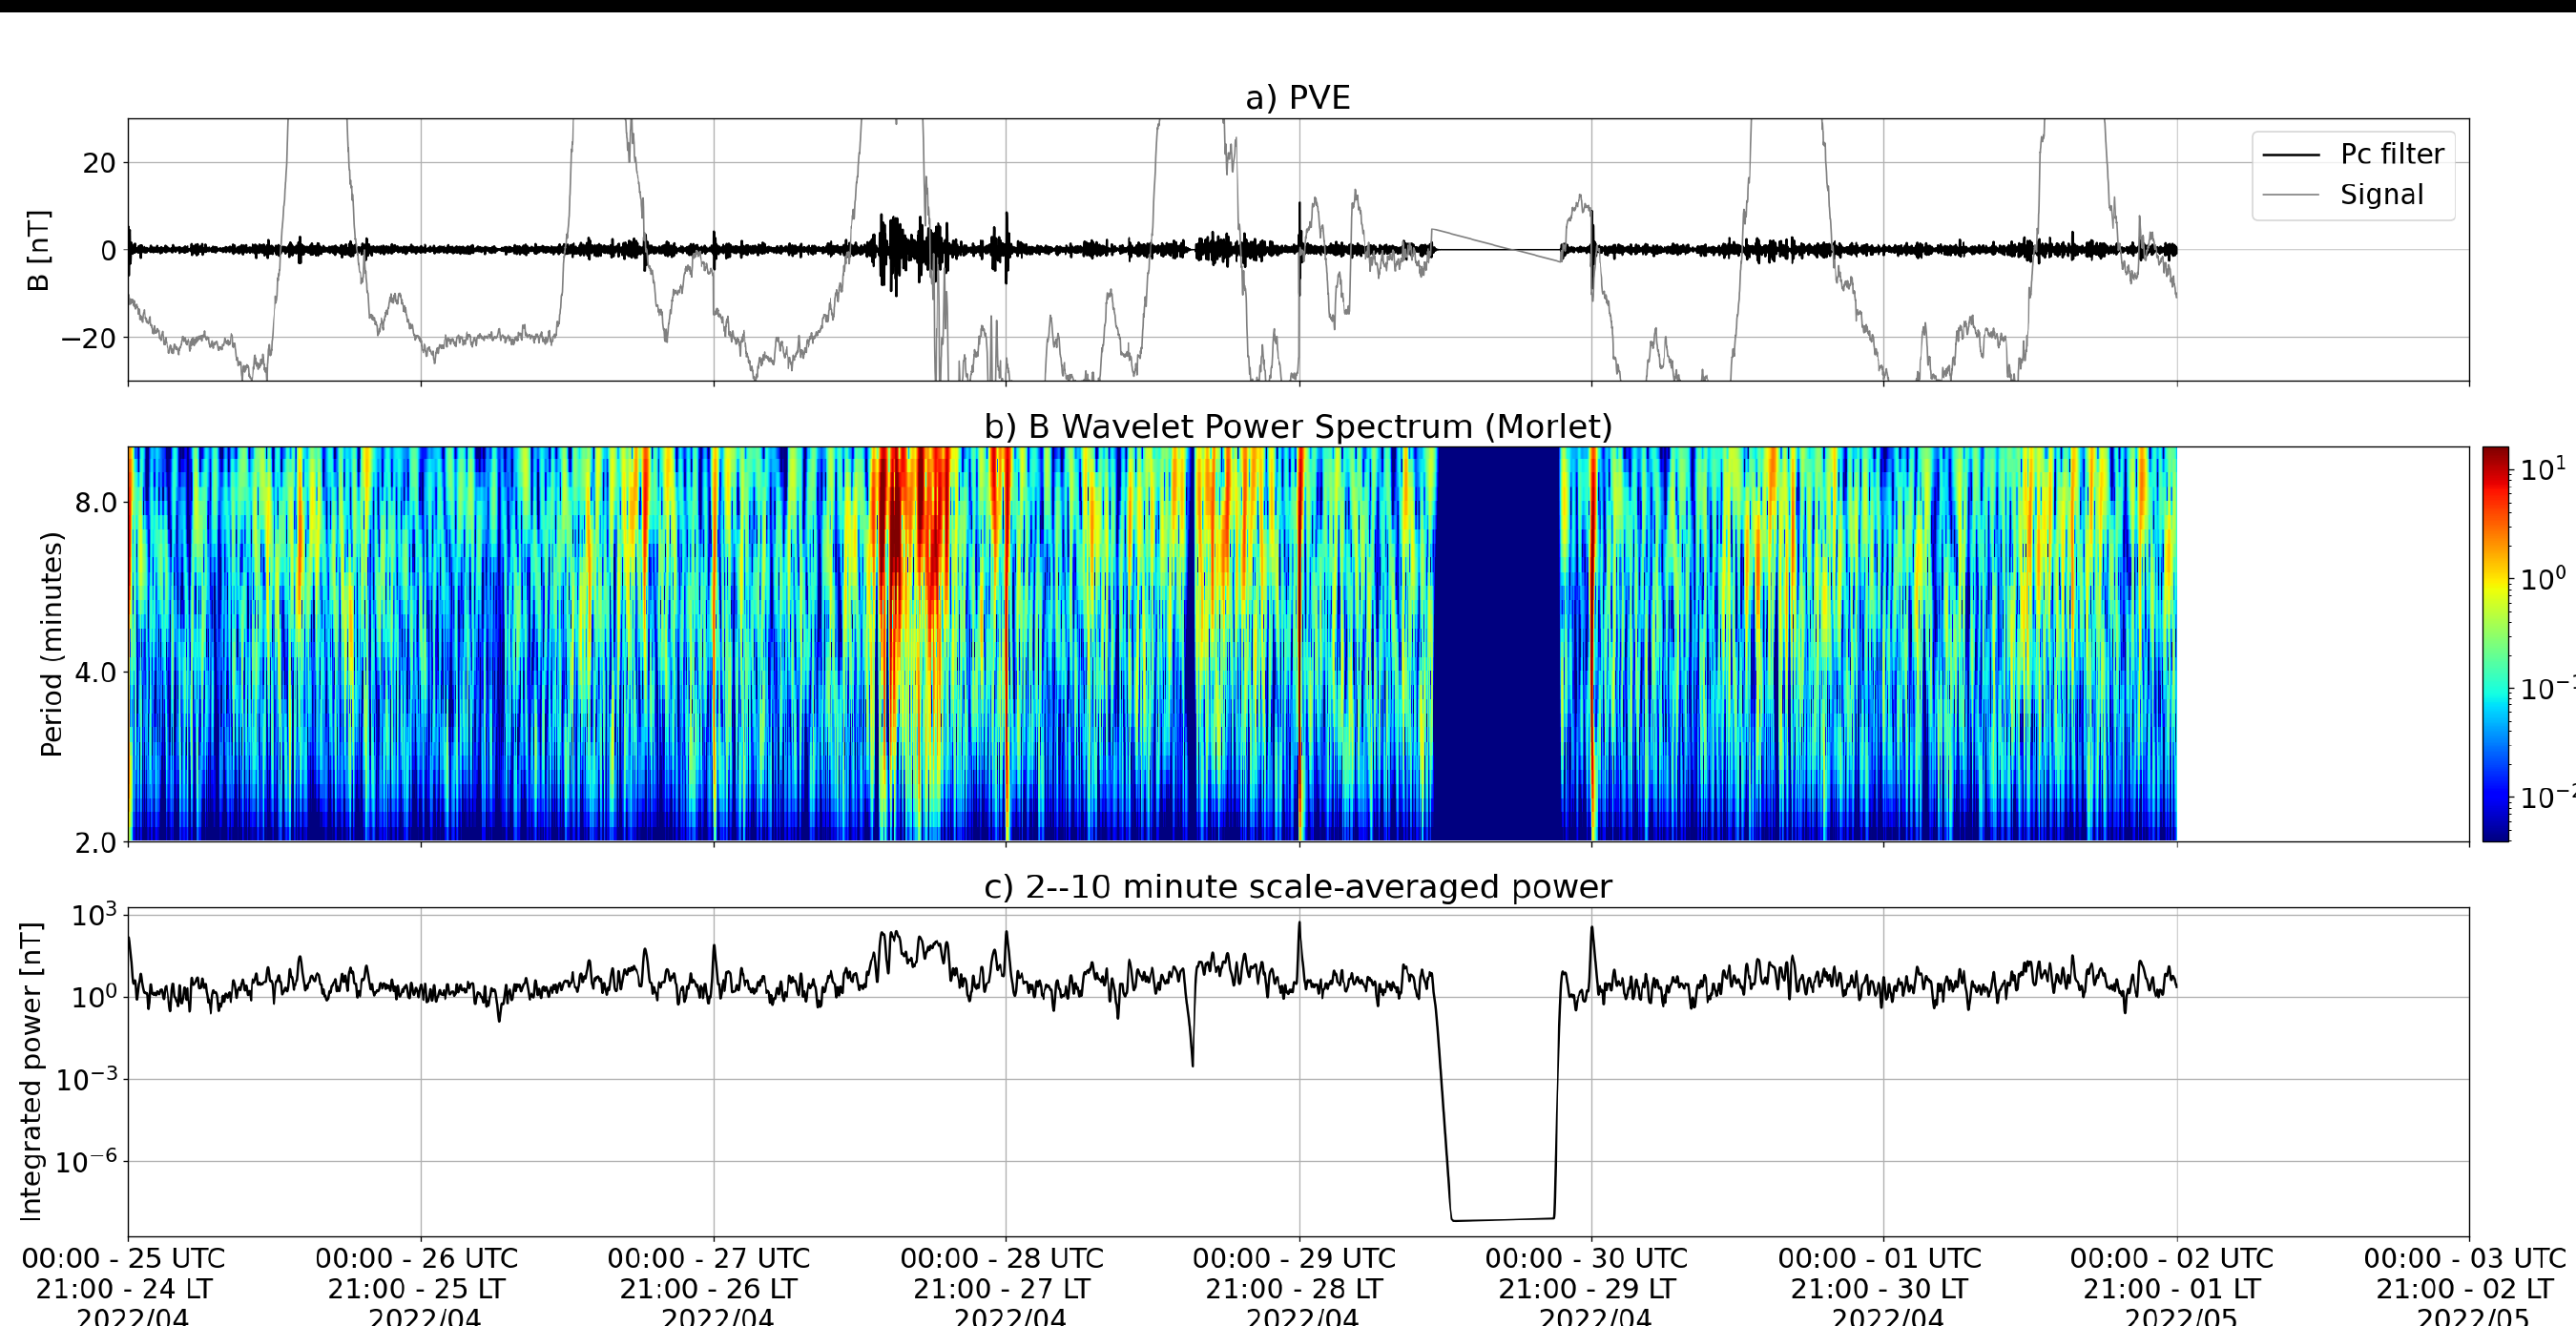
\includegraphics[width=14cm]{./figures//figureULF_1.png}

                             \caption{a) sinal do campo magnético total medido 
                              na Estação SMS da rede EMBRACE em cinza, junto com a 
                              flutuação na faixa de Pc5 em preto. b) Espectro de potência 
                              wavelet do sinal filtrado. c) Média da potência espectral nas 
                              faixas de 2 a 10 minutos (ondas ULF).}
                        \end{figure}

                     \begin{figure}[H]
    
                        \centering
   
                             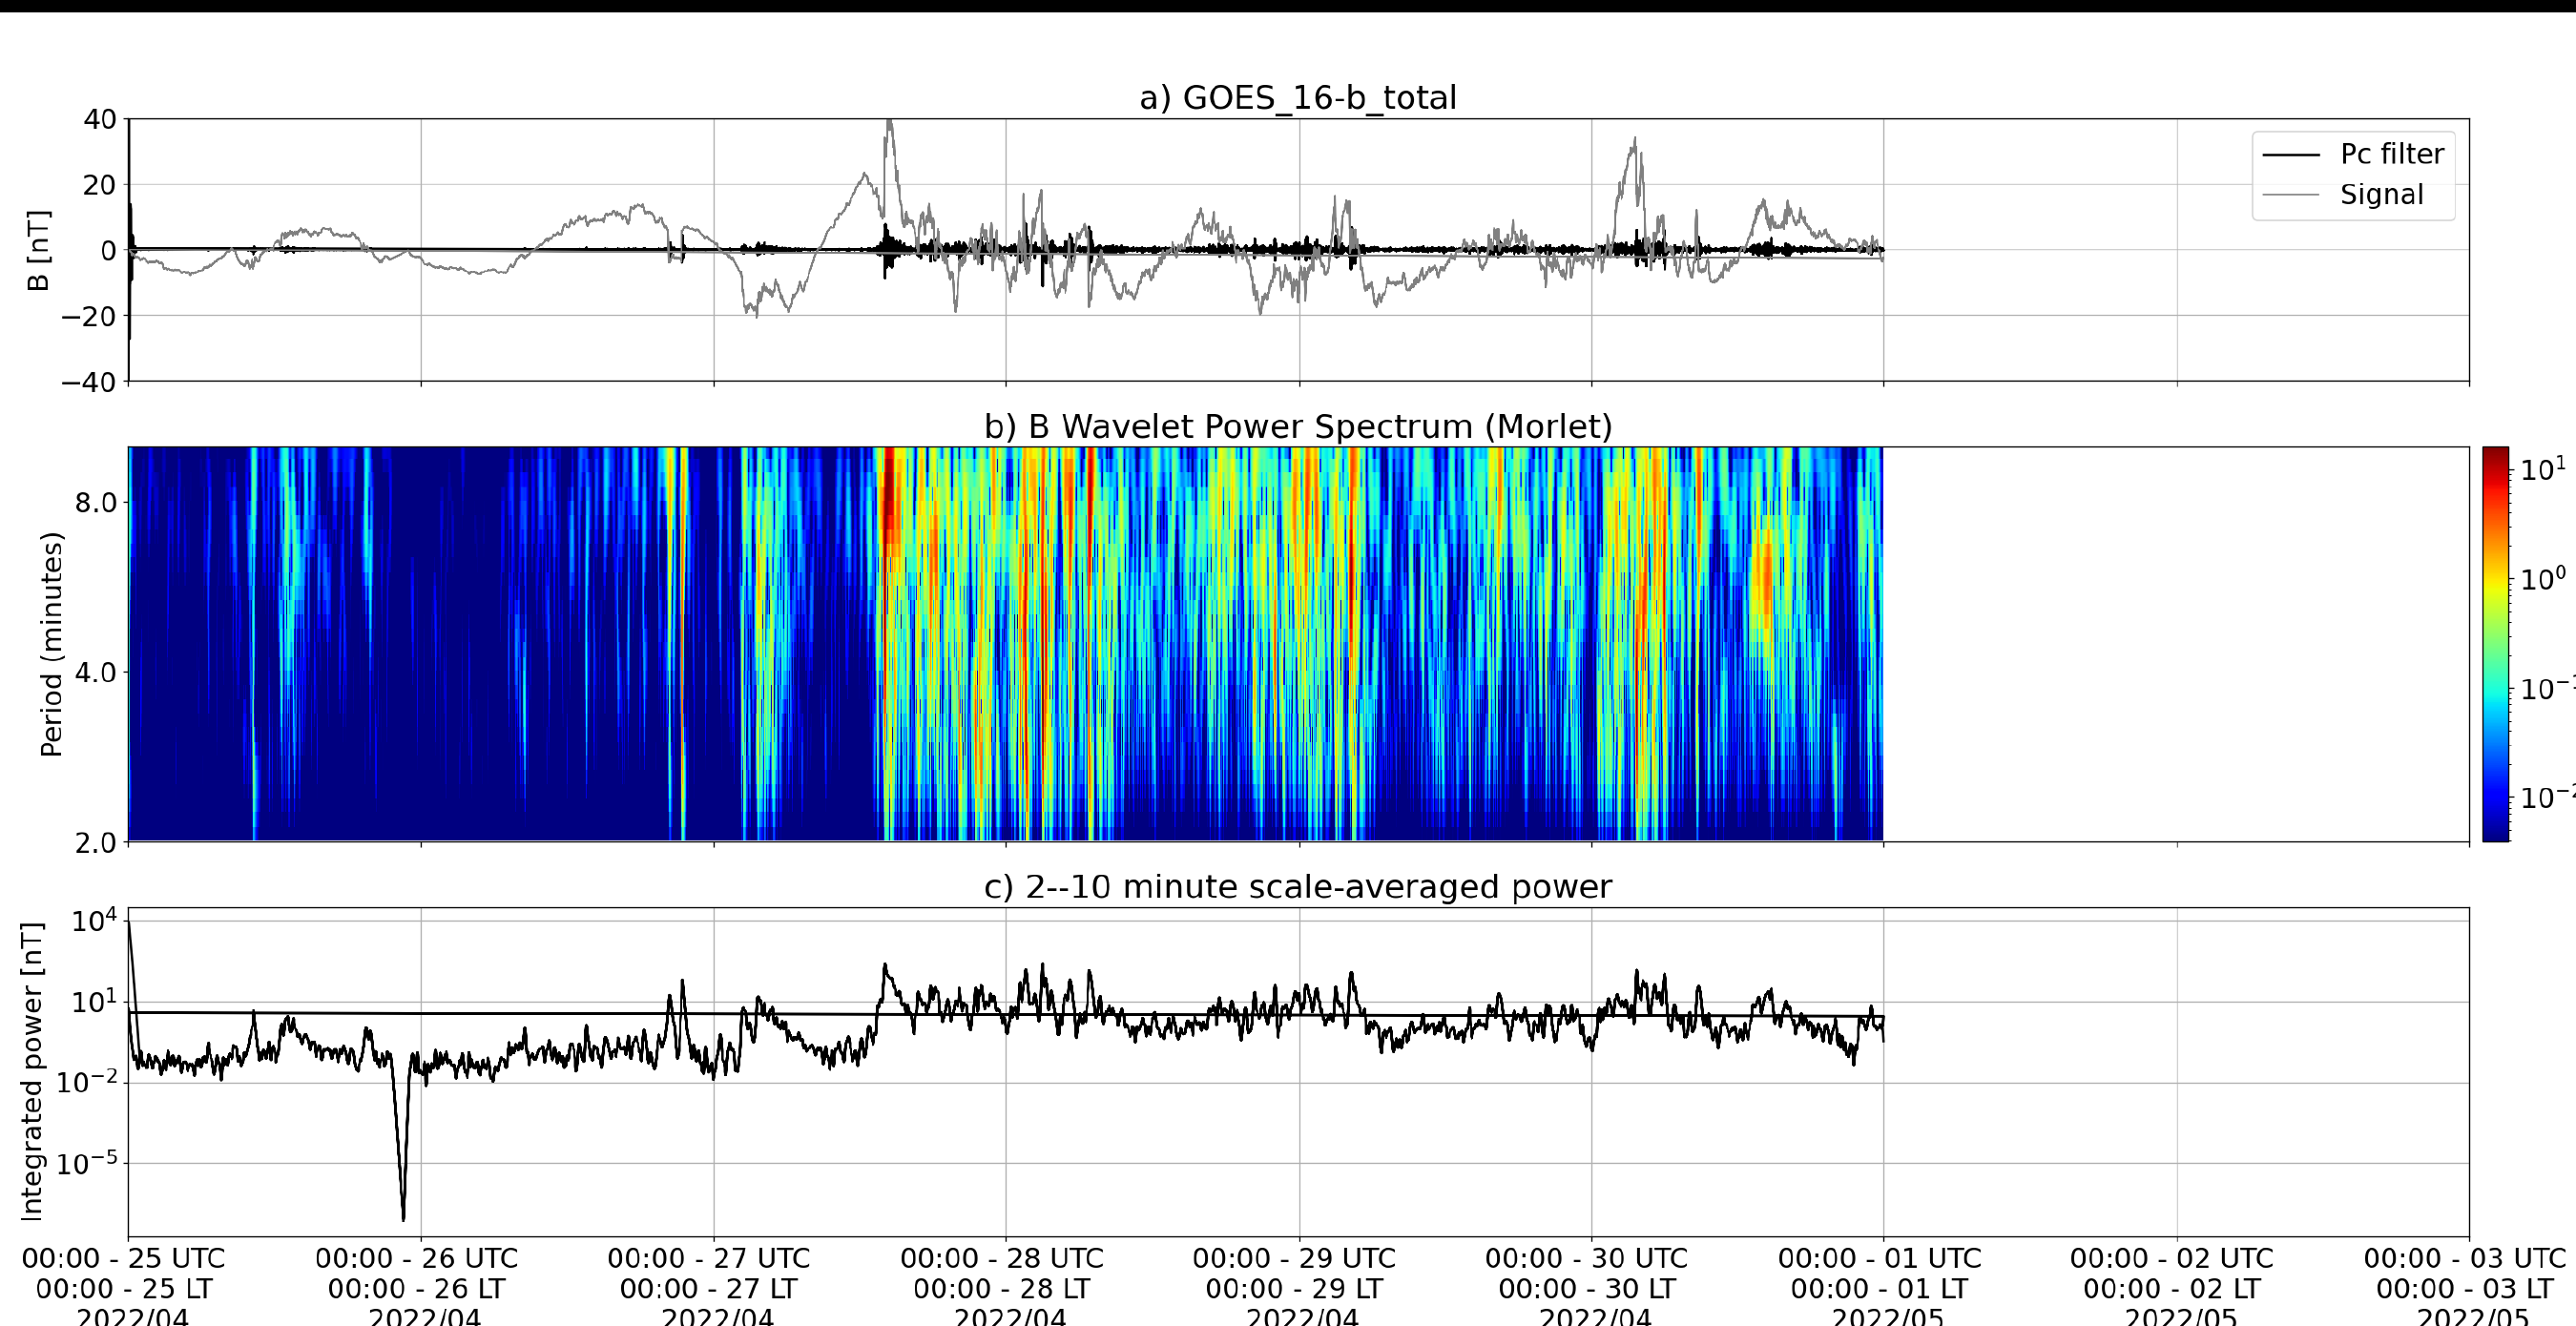
\includegraphics[width=14cm]{./figures//figureULF_2.png}

                             \caption{a) sinal do campo magnético total medido pelo 
                              satélite GOES 16, junto com a flutuação na faixa de Pc5 
                              em preto. b) Espectro de potência wavelet do sinal 
                              filtrado. c) Média da potência espectral nas faixas 
                              de 2 a 10 minutos (ondas ULF).}
                        \end{figure}

                     m A atividade de ondas ULF apresenta um aumento na potência a partir do
dia 3 de maio na forma de pulsações irregulares e de curta duração,
detectados desde altas latitudes até os magnetômetros em baixas latitudes
da rede EMBRACE (Figura 2, SMS), a mesma atividade se repete no dia 4 de
maio. A atividade continua até o dia 7 de maio com potência reduzida. No
dia 8 há um novo aumento na potência espectral, agora com características
contínuas, principalmente em altas latitudes. Esse período possivelmente
está sob o efeito de uma região de interação corrotante (CIR) e também
períodos com aumento da densidade do vento solar e componente do
campo magnético do vento solar predominantemente na direção sul.
Sumário
9/10
m A atividade de ondas ULF apresenta um aumento na potência a partir do dia 3 de maio na forma de pulsações irregulares e de curta duração, detectados desde altas latitudes até os magnetômetros em baixas latitudes da rede EMBRACE (Figura 2, SMS), a mesma atividade se repete no dia 4 de maio. A atividade continua até o dia 7 de maio com potência reduzida. No dia 8 há um novo aumento na potência espectral, agora com características contínuas, principalmente em altas latitudes. Esse período possivelmente está sob o efeito de uma região de interação corrotante (CIR) e também períodos com aumento da densidade do vento solar e componente do campo magnético do vento solar predominantemente na direção sul.\section{Ondas EMIC} 
 \subsection{Responsável: José Paulo Marchezi} 
 
\begin{figure}[H]
    
                        \centering
   
                             \includegraphics[width=14cm]{./figures//figureEMIC_1.png}

                        \end{figure}

                     \section{Geomagnetismo} 
 \subsection{Responsável: José Paulo Marchezi} 
 
\begin{figure}[H]
    
                        \centering
   
                             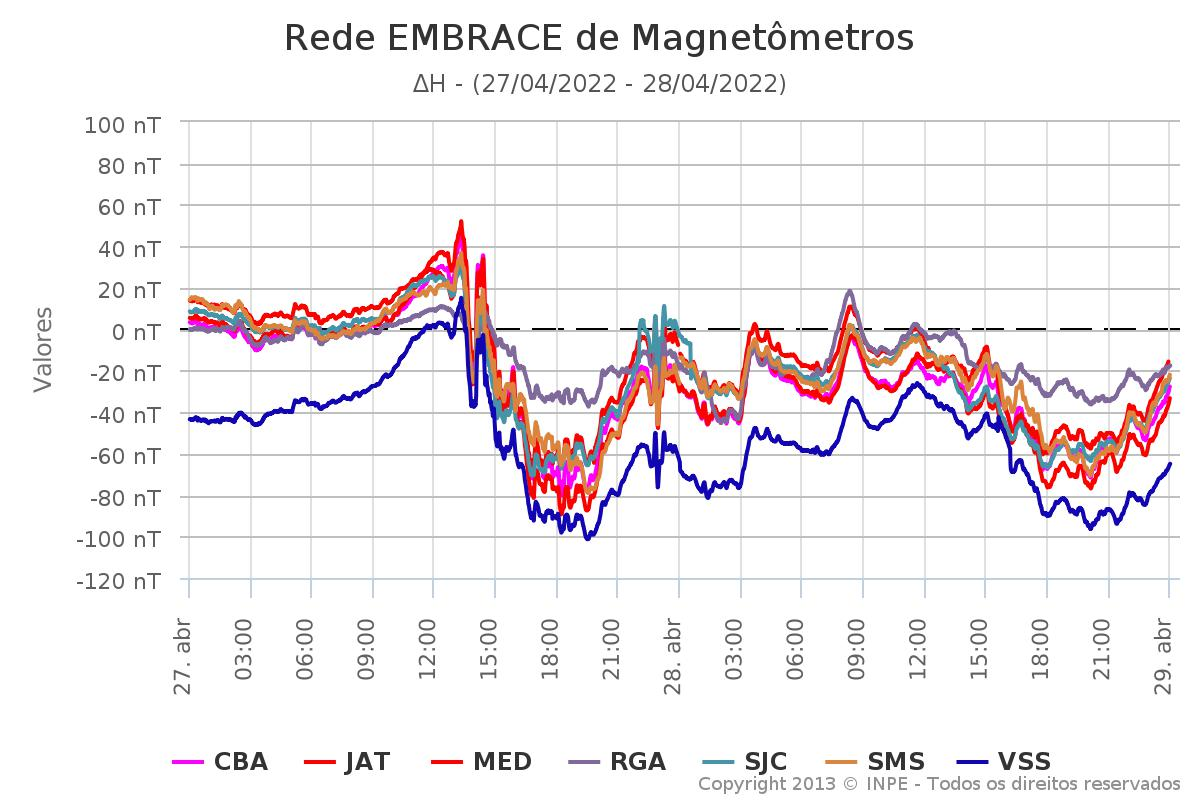
\includegraphics[width=14cm]{./figures//figureGeomag_0.png}

                        \end{figure}

                     \begin{figure}[H]
    
                        \centering
   
                             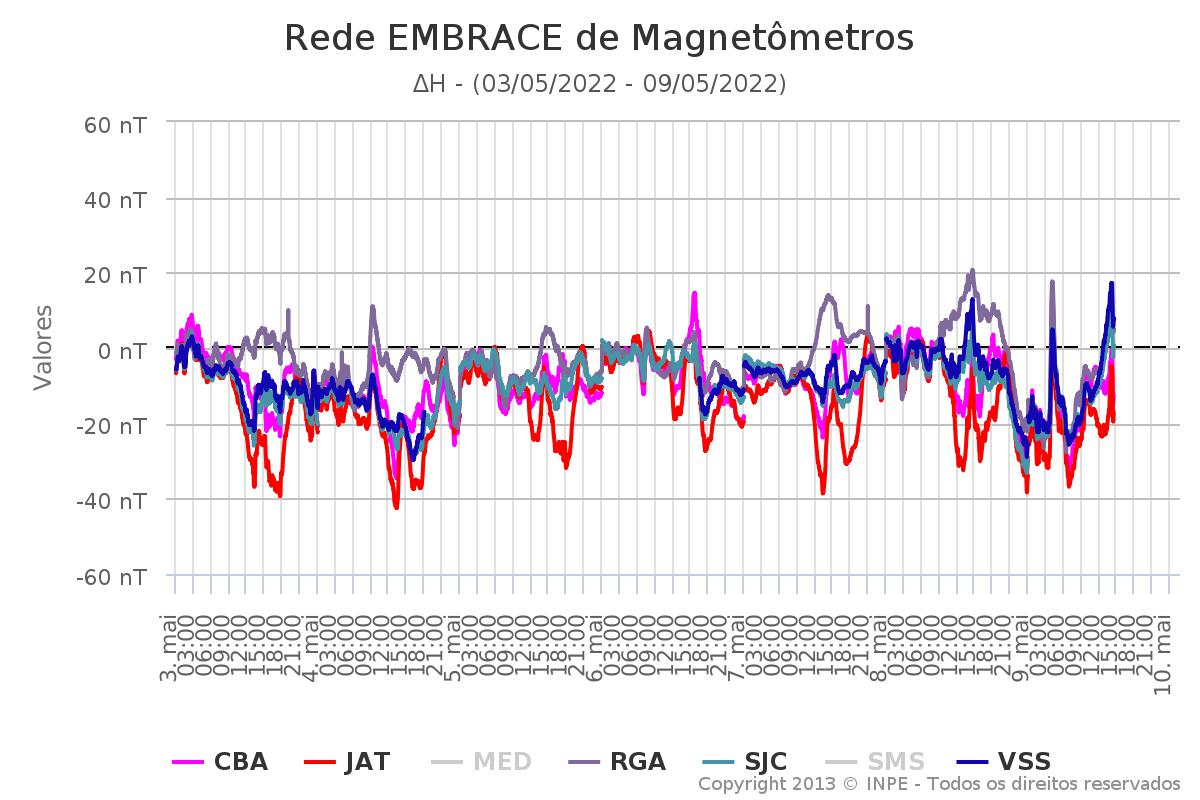
\includegraphics[width=14cm]{./figures//figureGeomag_1.png}

                        \end{figure}

                     \begin{figure}[H]
    
                        \centering
   
                             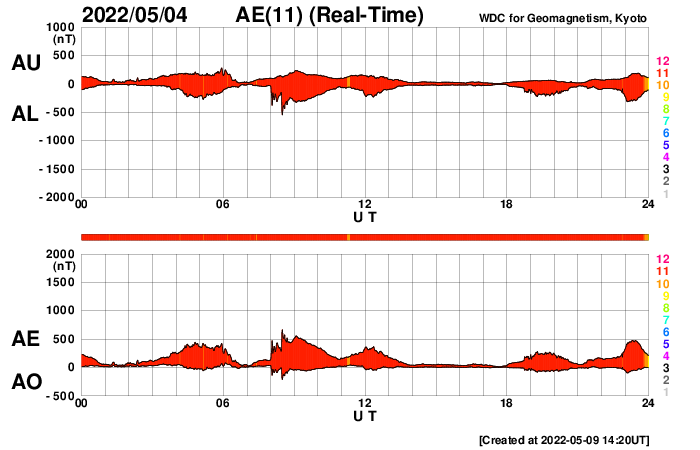
\includegraphics[width=14cm]{./figures//figureGeomag_2.png}

                        \end{figure}

                     \begin{figure}[H]
    
                        \centering
   
                             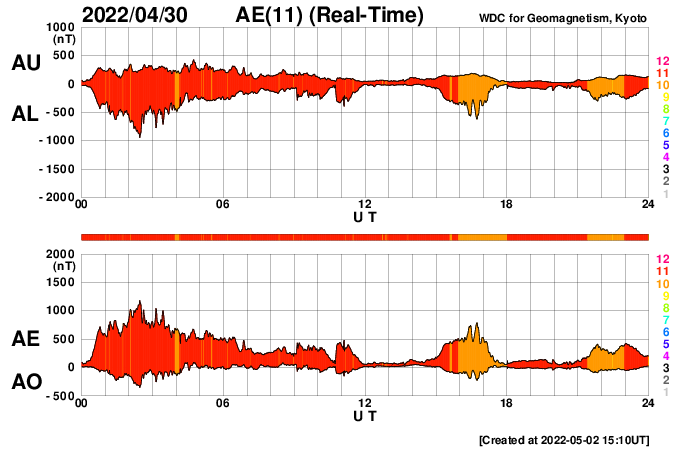
\includegraphics[width=14cm]{./figures//figureGeomag_3.png}

                        \end{figure}

                     \begin{figure}[H]
    
                        \centering
   
                             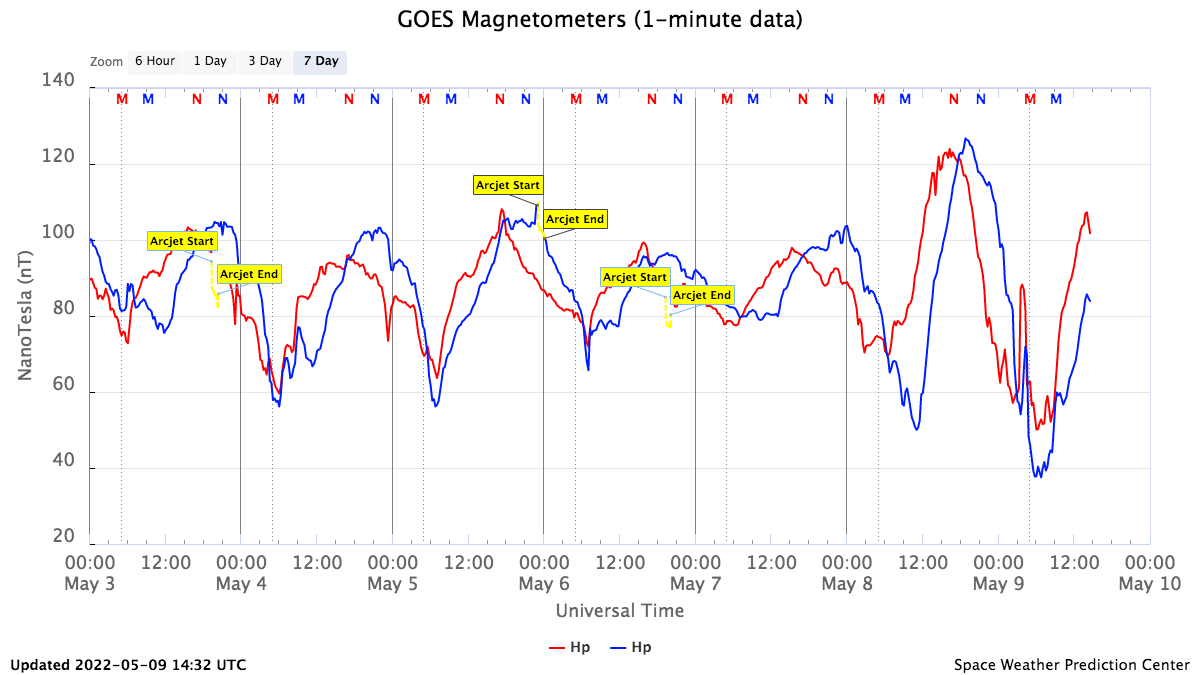
\includegraphics[width=14cm]{./figures//figureGeomag_4.png}

                        \end{figure}

                     \begin{figure}[H]
    
                        \centering
   
                             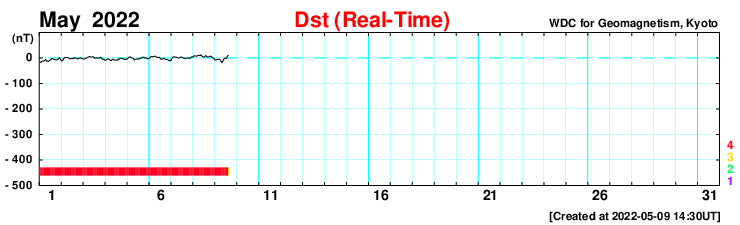
\includegraphics[width=14cm]{./figures//figureGeomag_5.png}

                        \end{figure}

                     \begin{figure}[H]
    
                        \centering
   
                             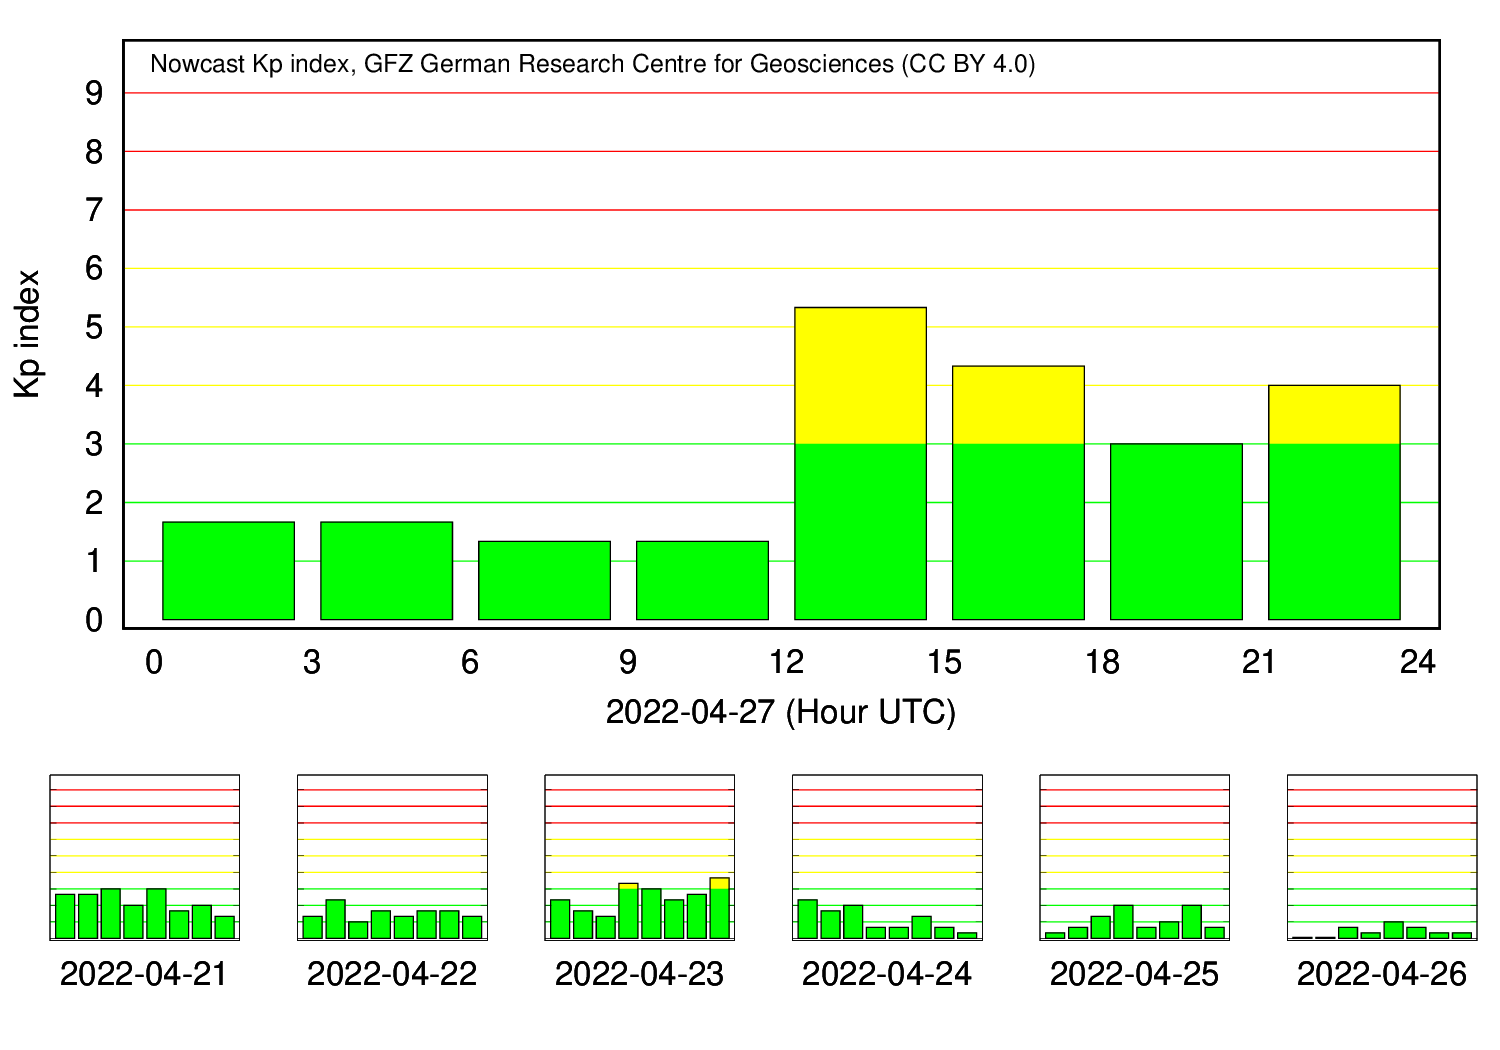
\includegraphics[width=14cm]{./figures//figureGeomag_6.png}

                        \end{figure}

                     \begin{itemize} 
\item Na semana de 03 a 09/05, destacam-se os seguintes eventos relacionados a atividade geomagnética:
\begin{itemize} 
 \item - Os dados provenientes da rede de magnetômetros Embrace apresentaram instabilidades durante todo o período, com alguns eventos em destaque:
 \end{itemize} 
\item As maiores perturbações na componente H foram registradas nos dias 03, 08 e 09 de maio
\begin{itemize} 
 \item - A atividade geomagnética foi instável durante todo o período, com o índice Dst oscilando em torno de zero. O Kp mais alto da semana foi de 3o
 \end{itemize} 
\begin{itemize} 
 \item - A atividade auroral foi levemente intensificada nos dias 09 e 04/05.
 \end{itemize} 
\begin{itemize} 
 \item - Campo magnético medido na órbita do satélite GOES apresentou perturbações no dia 09/05.
 \end{itemize} 
\end{itemize} 
\section{Ionosfera} 
 \subsection{Responsável: Laysa Resende} 
 
\textbf{Boa Vista: }

 \begin{itemize}
\item Ocorreu spread-F todos os dias.
\item As camadas Es atingiu a escala 4 no dia 07.
\end{itemize}
\begin{figure}[H]
    \centering
    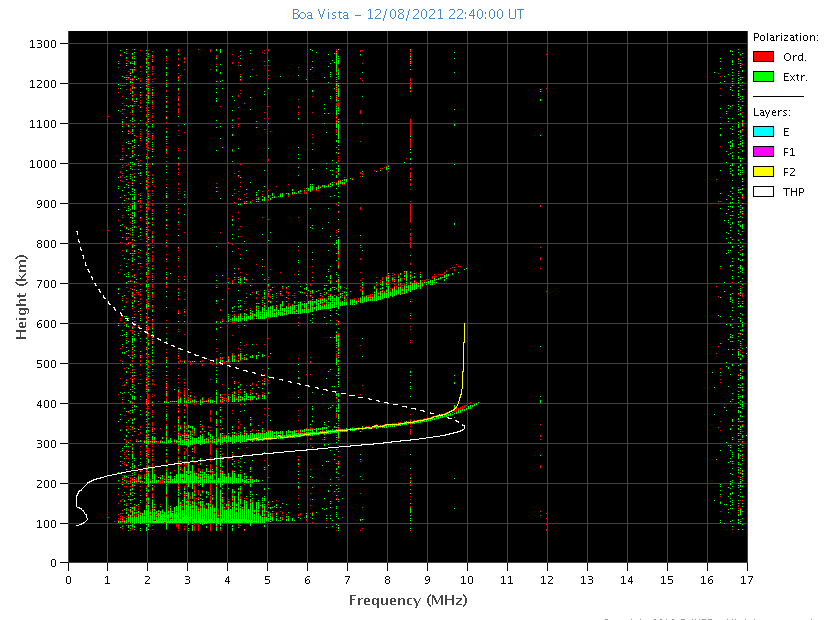
\includegraphics[width=14cm]{./figures//BoaVista.png}
\end{figure}

\textbf{Cachoeira Paulista:}

 \begin{itemize}
\item Não ocorreu spread-F durante a semana.
\item As camadas Es dessa região atingiu a escala 2 a semana toda. 
\end{itemize}
\begin{figure}[H]
    \centering
    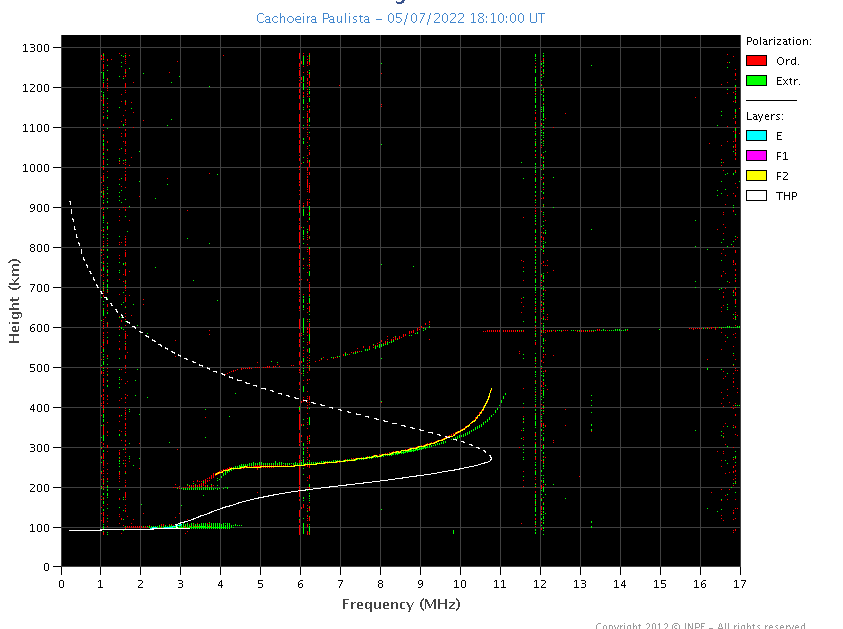
\includegraphics[width=14cm]{./figures//CachoeiraPaulista.png}
\end{figure}

\textbf{São Luís: }

 \begin{itemize}
\item Ocorreu spread -F durante toda a semana. 
\item As camadas Es dessa região atingiu a escala 4 no dia 05. 
\end{itemize}
\begin{figure}[H]
    \centering
    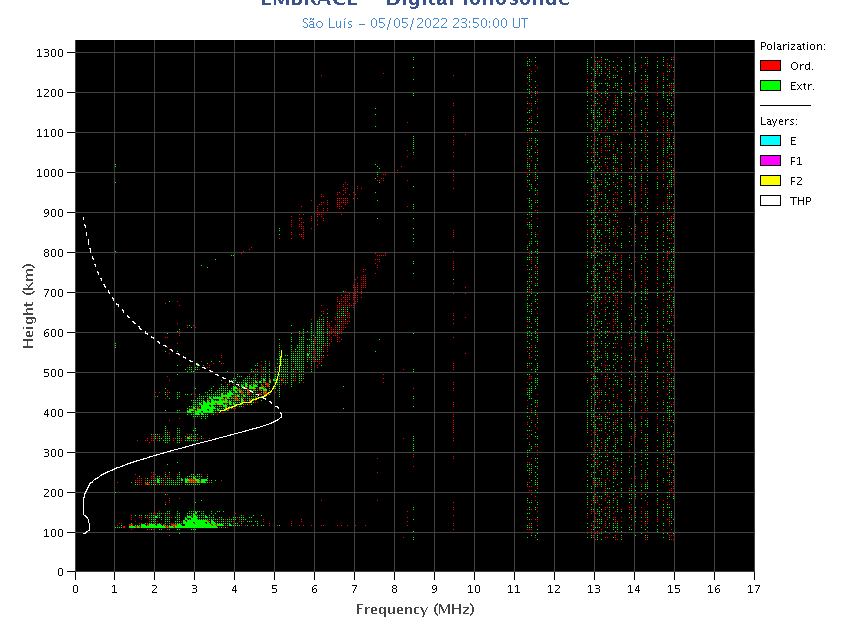
\includegraphics[width=14cm]{./figures//SãoLuís.png}
\end{figure}

\section{Cintilação} 
 \subsection{Responsável: Siomel Savio Odriozola} 
 
Neste reporte sobre o índice de cintilação S4, foram apresentados dados das 
estações FRTZ em Fortaleza/CE, STSN em Sinop/MG, UFBA em Bahía/BA e 
SJCE em São José dos Campos/SP. O índice S4 acompanha a presença de 
irregularidades na ionosfera quando elas têm uma escala espacial ~ 360 m.  
As estações STSN, STNT e SJCE não apresentaram valores relevantes do 
índice S4 durante toda a semana. Já na estação FRTZ, apareceu um caso com 
valores do S4 acima de 0.4 (Figura 1, painel superior) após a pôr do sol horário 
no dia 5/05. No painel inferior da Figura 1, aparecem os satélites afetados e que 
se encontram ao noroeste do FRTZ. Ionogramas no mesmo horário e local 
mostram o espalhamento no traço principal. Este fato junto com a posição dos 
satélites com valores do S4 > 0.15 mostrados na Figura 1 indicam a presencia 
de uma irregularidade no plasma ionosférico devido a uma bolha de plasma 
típica em este horário e em estas latitudes próximas a o equador geomagnético. 

    \begin{figure}[H]
        \centering
        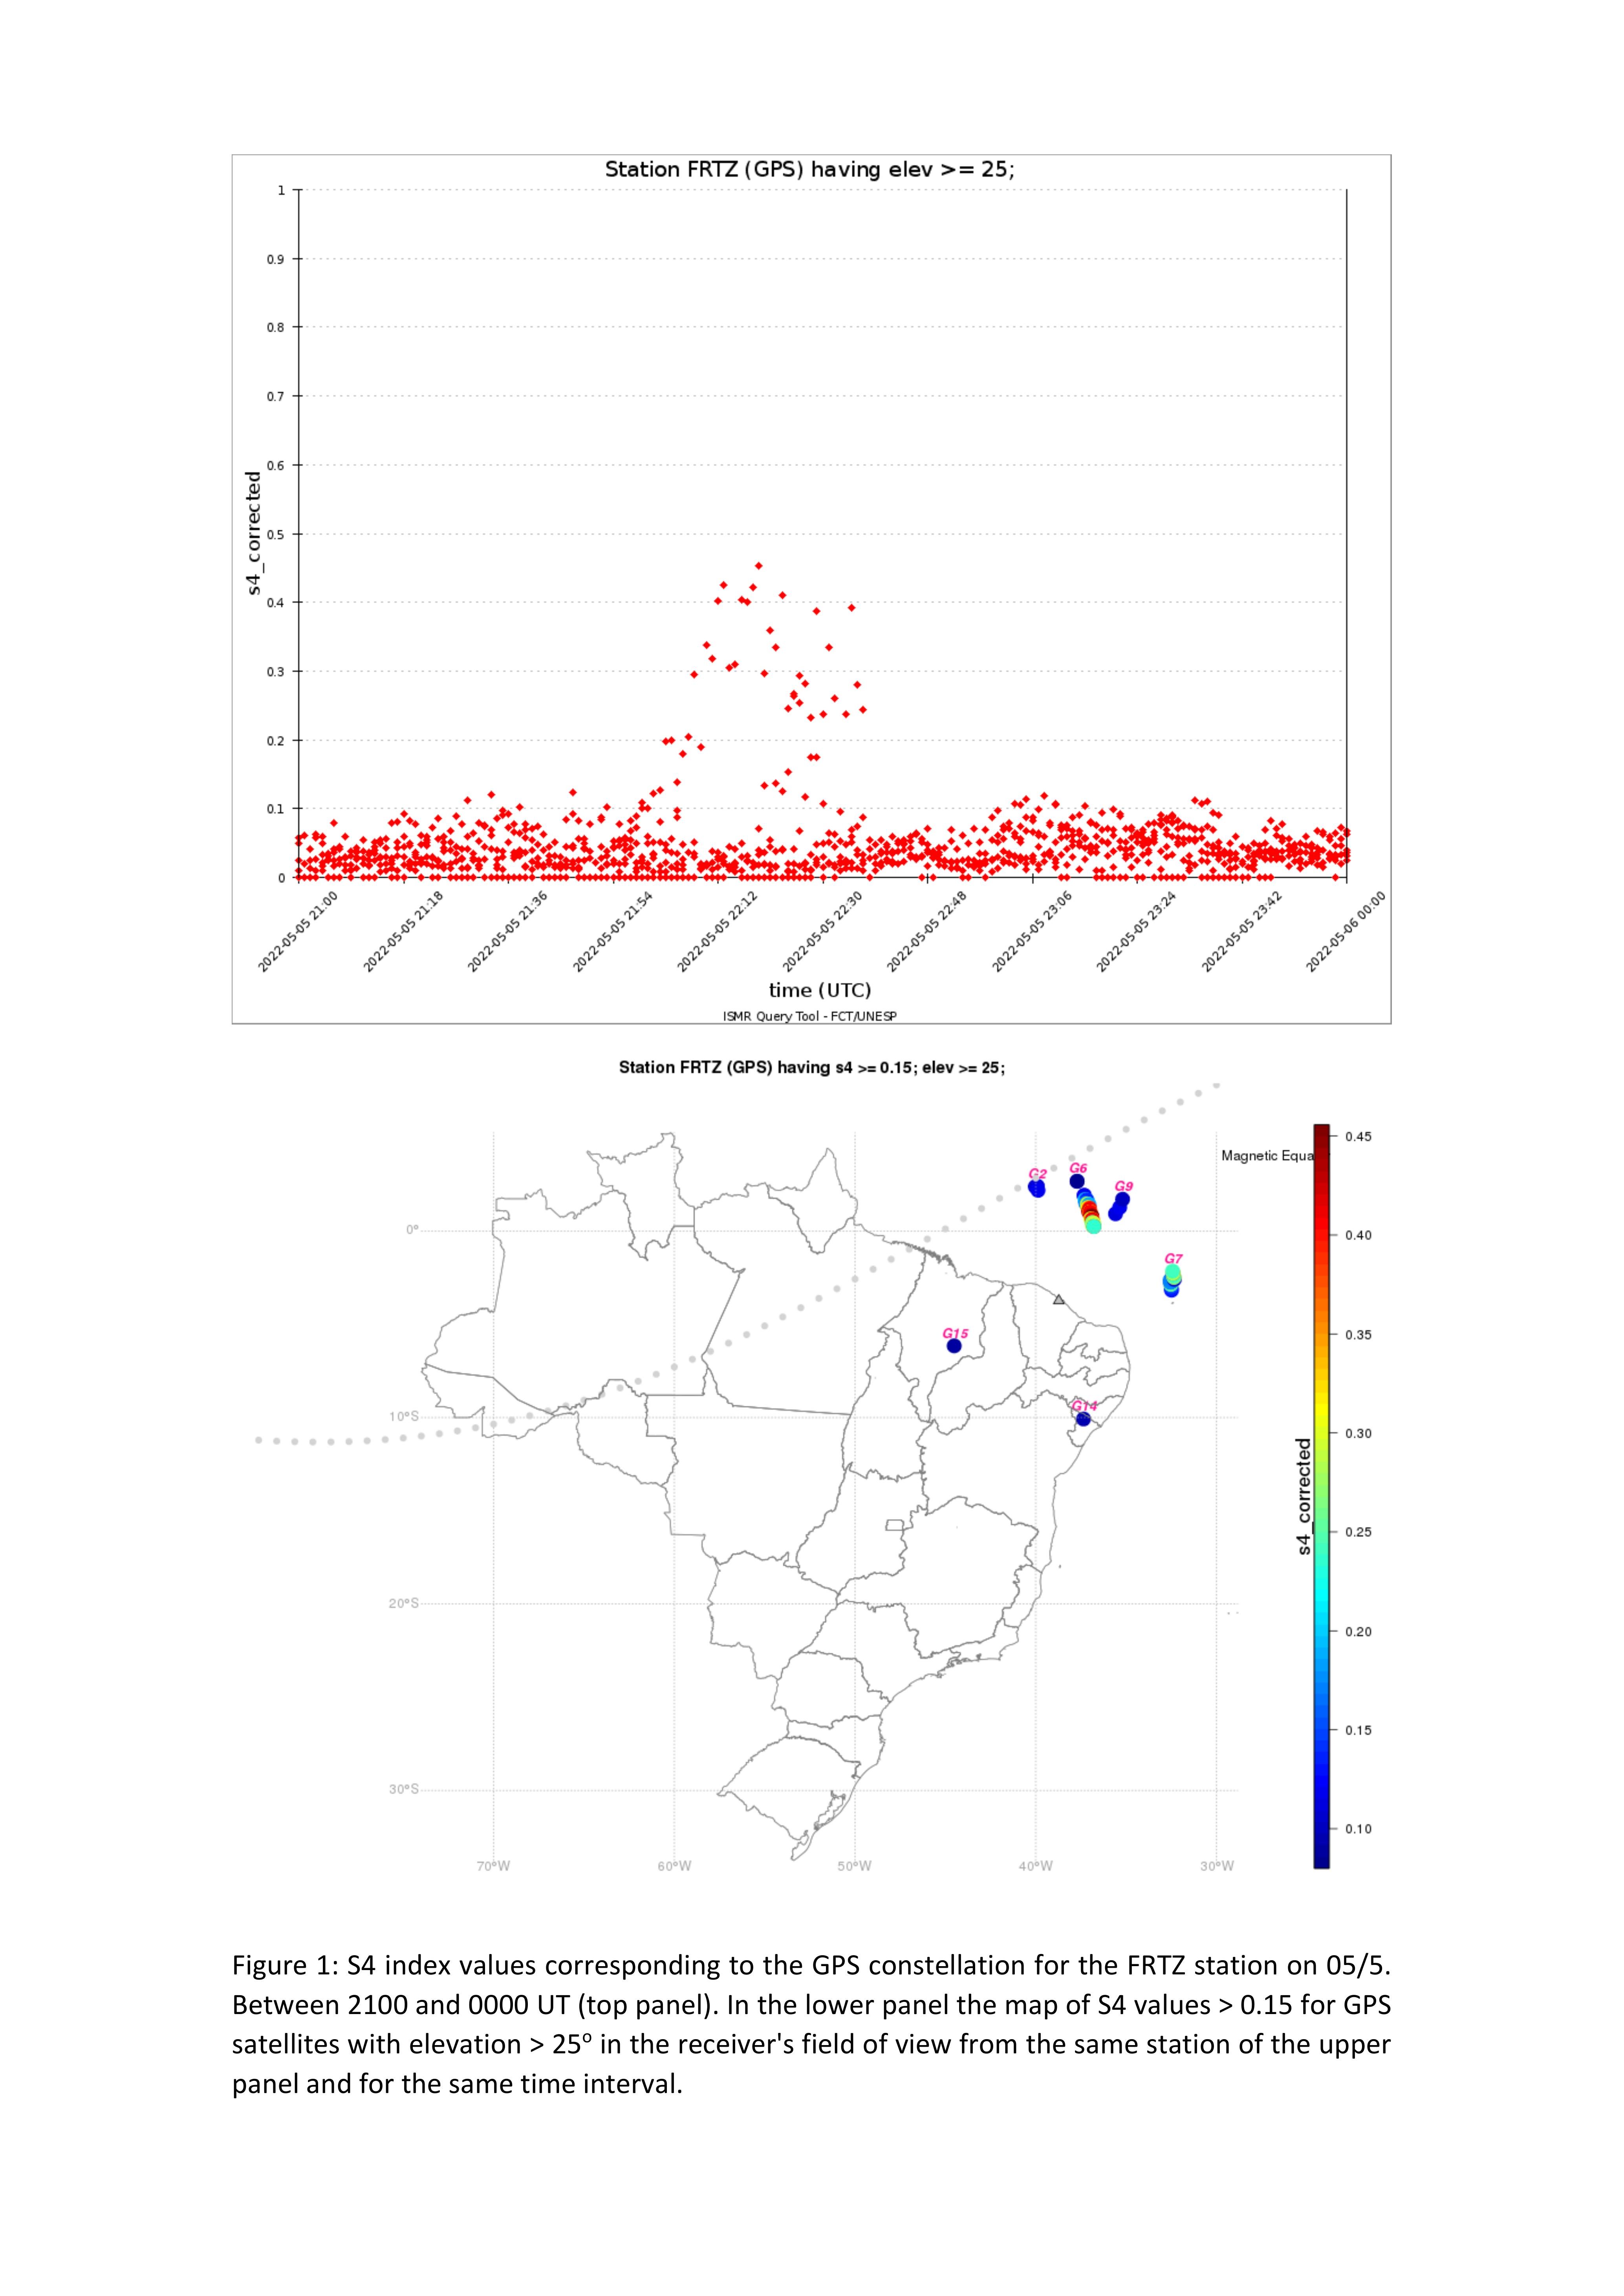
\includegraphics[width=14cm]{./figures/pt_outfileScint_0.jpg}
    \end{figure} 
 

    \section{ROTI} 
 \subsection{Responsável: Carolina de Sousa do Carmo} 
 
O ROTI não apresentou significativas variações relacionadas com irregularidades ionosféricas no decorrer da semana. Porém, é interessante mencionar que apareceram algumas estruturas na região norte do Brasil em todos os dias da semana. Contudo, esta região possui baixa cobertura espacial de receptores GNSS e há também os efeitos de bordas nos mapas, fazendo com que haja uma propagação de erros nessa região específica.



\end{document}